\documentclass[runningheads,a4paper]{llncs}

\usepackage{amssymb}
\setcounter{tocdepth}{3}
\usepackage{graphicx}

\usepackage{url}

\urldef{\mailsa}\path|{radiceadriann, facundosanabria}@gmail.com|    
\newcommand{\keywords}[1]{\par\addvspace\baselineskip
\noindent\keywordname\enspace\ignorespaces#1}

\newcommand{\MR}{$\emph{MatulaRubik}$ } 

\begin{document}

\mainmatter  % start of an individual contribution

% first the title is needed
\title{Trabajo de Investigación:\\
Integración de HPC en IOT}

% a short form should be given in case it is too long for the running head
\titlerunning{Investigación: HPC y Rubik}

% the name(s) of the author(s) follow(s) next
%
% NB: Chinese authors should write their first names(s) in front of
% their surnames. This ensures that the names appear correctly in
% the running heads and the author index.
%
\author{Adrian Radice%
\and Facundo Sanabria}
%
\authorrunning{Investigación: HPC y Rubik}
% (feature abused for this document to repeat the title also on left hand pages)

% the affiliations are given next; don't give your e-mail address
% unless you accept that it will be published
\institute{Universidad Nacional de La Matanza,\\ Departamento de ingeniería e Investigaciones Tecnológicas,\\
Florencio Varela 1903 - San Justo, Argentina\\
\mailsa\\
\url{http://www.github.com/BitesellerSOA}}

%
% NB: a more complex sample for affiliations and the mapping to the
% corresponding authors can be found in the file "llncs.dem"
% (search for the string "\mainmatter" where a contribution starts).
% "llncs.dem" accompanies the document class "llncs.cls".
%

\toctitle{Lecture Notes in Computer Science}
\tocauthor{Authors' Instructions}
\maketitle


\begin{abstract}
El objetivo del presente trabajo es investigar los beneficios de incorporar HPC en el proyecto de IOT
\MR. Dicho proyecto tiene como desafío resolver un problema NP. Este problema es el puzzle Rubik 3x3x3, el cual
se solucionara implementando el algoritmo no determinístico CFOP. CFOP varia de acuerdo cual 
se su cara de partida, por lo tanto para cualquier cubo se tienen 6 estados iniciales. El desafío es de 6 posibles caminos para 
llegar al estado final, quedarse con aquel que implique el menor uso del brazo lateral.
\keywords{HPC, IOT, Android, Rubik, Paralelismo, OpenCL}
\end{abstract}


\section{Introducción}
\MR es un SE con el objetivo de resolver el Cubo Rubik de 3x3x3, en una primera instancia aplicando el algoritmo utilizado para competencias de velocidad CFOP, el cual obtiene un promedio entre 50 y 100 movimientos para resolver cualquier cubo.
Este algoritmo pertenece a la familia de los llamados \emph{Layer by Layer}, y se caracteriza por llevar a cualquier configuración del cubo a un estado particular, reduciendo siempre 
al problema a la misma solución. En pocas palabras mezcla aun mas el cubo para llevarlo a estados conocidos. 
CFOP es un algoritmo en donde un estado tienen distintas transiciones que nos llevan al estado final, siendo 
cada una finalmente un camino con distinta o igual cantidad de movimientos. 


El objetivo de esta investigación, es reducir el tiempo en que \MR  entrega la solución. \MR  actualmente en su mecánica, 
tiene un retardo extra, la ubicación de las caras laterales en el correspondiente brazo para poder rotarlas. Se buscara mediante
la implementación de HPC con OpenCL, encontrar la solución que reduce el retardo previamente descrito.

\section{Desarrollo}

Estudiando la mecánica de \MR se aprecia que el efectuar movimientos en las caras L, F, R, B pueden sumar un retardo, que no existe nunca al trabajarse con las caras U y D. Por ejemplo la secuencia de movimientos F, B' implica, que luego de ejecutarse el primer movimiento, se sume un retardo temporal hasta que la cara B del cubo quede frente al brazo. Este retardo es el tiempo que implica retirar el brazo lateral, rotar el cubo hasta que B quede frente del brazo, y que el brazo lateral se ubique nuevamente en la posición de trabajo.

Enfrentar dicho problema implicaría dos caminos,  cambiar la mecánica, o buscar una reducción en los movimientos de las caras problemáticas. En el desarrollo del trabajo optaremos por el segundo camino.

\MR en su estado actual aplica el algoritmo CFOP, el mismo presenta la particularidad que para una misma configuración del cubo de acuerdo a la cara que se tome como punto de partida devolverá una secuencia de movimientos totalmente distinto. Es decir, es como si se rotase lógicamente el cubo respecto de uno de sus ejes, lo que provoca que todas las piezas cambien de posición y orientación, resultando en un estado desordenado distinto y por lo tanto el algoritmo devolverá un conjunto de movimientos completamente distinto.


Para lograr obtener la menor cantidad de movimientos posibles utilizando este algoritmo nos proponemos a ejecutar en forma paralela 6 hilos de CFOP, un hilo por cara del cubo.

En busca de no tener que modificar demasiado el código actualmente implementado, se busco una herramienta que implique una implementación sencilla y optima de paralelismo. La herramienta seleccionada fue Paralldroid.

Paralldroid es un framework de desarrollo, que tiene como objetivo facilitar el trabajo de los desarrolladores de aplicaciones móviles ejecutadas sobre sistemas operativos Android, de acuerdo a lo mencionado en "Performance Analysis of Paralldroid Generated Programs" \cite{jour}. El mismo añade un conjunto de anotaciones al lenguaje Java, basadas en las definidas por el estándar OpenCL, permitiendo al desarrollador usar un lenguaje de alto nivel, sin entrar en detalle de implementación de paralelismo, y delegandole la responsabilidad a Paralldroid de generar el programa paralelo, segun lo indicado en "ParallDroid: A Framework for Parallelism in Android" \cite{bookParalldroid}.
Paralldroid puede ser descargado como plugin para eclipse, y solo es necesario instalarlo para que comience a funcionar\cite{jour}.


\begin{figure}
\centering
        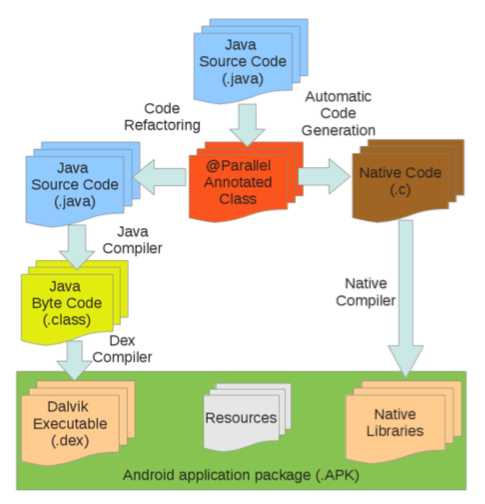
\includegraphics[totalheight=4cm]{Modelo.png}
        \caption{Resultado de la refactorización \cite{OpenCLbook}.}
\end{figure}

Como se puede apreciar en la Figura 1 este framework, mediante el código Java con anotaciones, obtendrá un código nativo OpenCL, invocado desde nuestras clases. Es elemental el uso de NDK en cualquier App para poder hacer uso de este framework.

\section{Distribución de operaciones}
La particularidad de los hilos de trabajos propuestos, es que son independíentes entre si, cada uno trabaja con su propia matriz de estado del cubo, sin intervenir con los otros. Partiendo de que el resultado de ParallDroid es una implementación de OpenCL \cite{jour}, cada hilo tendrá destinado un WorkGroup independíente. La primera ventaja de esta división, es que cada WorkGroup podrá ser ejecutado en una unidad de procesamiento distinta, si OpenCL lo considera \cite{OpenCLbook}, y como segunda ventaja es el escalado automático (asignación de WorkGroup a las unidades de procesamiento) que implementa OpenCL \cite{OpenCLbook}. Esta ultima ventaja hace referencia, a que un mismo código, en un dispositivo de mayor cantidad de unidades de procesamiento que WorkGroups, en el mejor de los casos cada  se asignara un WorkGroup por unidad de procesamiento, y en un dispositivo de menor cantidad,  OpenCL simplemente terminaría ejecutando un conjunto de los WorkGroups en serie, en las unidades de procesamiento disponible.


\section{Explicación Algoritmo}

Nos basamos en el típico ejemplo de paralelismo del producto entre un escalar y un vector. Buscar 6 soluciones es isomórfico a esto 
ultimo, si entendemos al resultado de la operación como un conjunto de 6 elementos. 

\medskip
\noindent
{\it Pseudocódigo}
\begin{verbatim}
@Parallel
public class SolverHPC_CFOP {
  private caras[];
  private  Solucion[];
 @Kernel
  private void Solver(CaraInicial){
         //CALCULAMOS LA SOLUCION
         Solucion [CaraInicial] <- CFOP(caraInicial);
  }
  private Solucion getBest(){
 	//SE CALCULA LA MEJOR SOLUCION
 	return Solucion[bestSol];
  }
}
public class Solver{
   SendSol(){
   	SendArduino(SolverHPC_CFOP.getBest());
   }
}
\end{verbatim}
%
\noindent

Según lo mencionado en "Performance Analysis of Paralldroid Generated Programs" \cite{jour}, ParallelDroid al refactorizar el código, agregaría el manejo de hilos, y nos abstrae de su desarrollo.



\section{Pruebas que pueden realizarse}
Para probar el rendimiento se propone, el desarrollo de un programa probador que mida el tiempo que le implica resolver 50 estados desordenados distintos del  puzzle a a MatulaRubik con HPC y luego sin HPC. A partir de estos resultados debería realizarse el promedio para ambos casos y comparar cual obtiene el mejor tiempo.

También seria útil comprobar que el conjunto de movimientos resultados sean distintos dependiendo por que cara se comienza y si difieren mucho entre ellos.

\section{Conclusión}

La fortaleza de la solución propuesta en la investigación, es que permite una implementación de paralelismo sin demasiado esfuerzo de desarrollo. Se aprovecha el poder computacional provisto por el Hardware de los dispositivos móviles, para contrarrestar una deficiencia mecánica. 

Extender la propuesta a cada uno de los distintos estados de CFOP en lugar de solamente los 6 iniciales seria computacionalmente intratable dado que CFOP es un algoritmo no determinístico, con una excesiva cantidad de estados posibles. Se compensaría los retrasos impuestos por la mecánica, con el tiempo de la búsqueda de mejor solución. 


\begin{thebibliography}{4}
\bibitem{jour} A. Acosta and F. Almeida, "Performance Analysis of Paralldroid Generated Programs" 2014 22nd Euromicro International Conference on Parallel, Distributed, and Network-Based Processing, Torino, 2014, pp. 60-67.
\bibitem{bookParalldroid} Vicente Blanco, "ParallDroid: A Framework for Parallelism in Android".
\bibitem{OpenCLbook} Aaftab Munshi, "The OpenCL Specification" Khronos OpenCL Working Group, Revision 2015.
 \end{thebibliography}
\end{document}
